%\section{Prediction Evaluation}
Recall from Section 2.4 that a receiver operating characteristic (ROC) curve is a metric for the ability of a classifier to discern between classes, where a larger area under the curve indicates better predictive performance. The y-axis is the true positive rate (sensitivity) and the x-axis is the false positive rate (1 - specificity). In this chapter, we discuss the changing predictive ability of our classifier as it went through various iterations visualized through ROC curves on four distinct validation sets.

%"state space of a column" is a little unclear to me. What is a column here? an example might aid the section
Each of the ROC curves below were generated using the required percent of random forests in the ensemble to flag a contest as a positive for it to be labeld as a positive as the threshold. (Once again, a flagged contest is one that will not fill to its target entries within the time that it is open to entries). Since our ensemble used 20 forests, each ROC was made from 20 threshold values. A ROC curve representing an optimal algorithm will flag every True Positive (TP) contest without flagging a single False Positive (FP). It is nearly impossible to create an algorithm with perfect sensitivity and specificity, so our goal was simply to maximize the area below the ROC curve. 
In the following graphics, many of the ROC curves are rainbow colored. This coloring is to help identify the threshold used to produce the indicated TP and FP rate.

\begin{figure}[h]
\centering
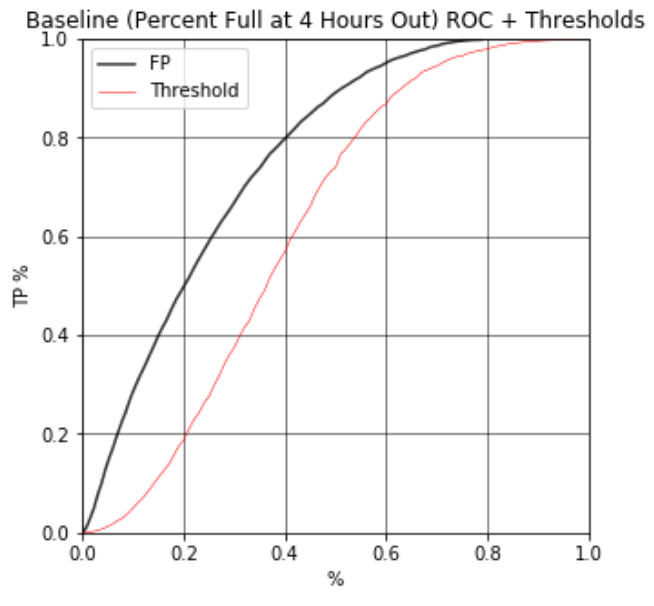
\includegraphics[width=6cm]{body/results/baseline.png}
\caption{ROC generated predicting solely based on how much each contest had already filled by the ``4 Hours Remaining'' point. This represents an initial baseline estimation we needed to outperform.}
\label{fig:baseline}
\end{figure}

To ensure we weren't over-complicating our approach, our first step was to generate a simple baseline ROC curve. Figure \ref{fig:baseline} was generated for this purpose by moving the threshold through the column, ``Percent Full at 4 Hours Out''. At a threshold of 50\%, any contest which was less than 50\% full at the Time Series data point 4 hours before contest start was flagged as a positive. At that threshold, approximately 80\% of True Positives are flagged with only 40\% of False Positives flagged. This visual is a good way of showing the data-set is inherently highly imbalanced as it would seem we can achieve a decent prediction by simply evaluating each contest at the ``4 Hour Out'' mark with no need for a complicated prediction.
%it would be dope if you could actually put the points on the graph for your example but don't worry too much for this draft

\begin{figure}[h]
\centering
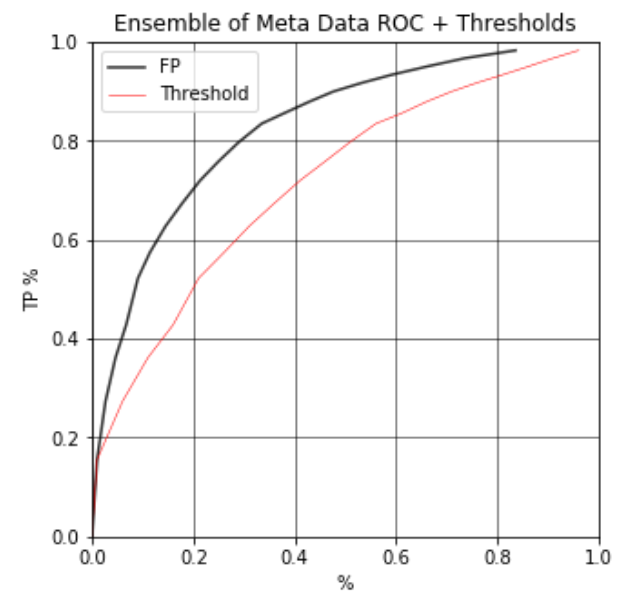
\includegraphics[width=6cm]{body/results/ensMet.png}
\caption{ROC generated based on an ensemble of random forests using only provided Header data.}
\label{fig:metaonly}
\end{figure}

Figure \ref{fig:metaonly} was generated using Meta data in a Random Forest Classifier (RFC) ensemble. A single RFC classifies True or False (1 or 0), which would limit the number of potential threshold values to only two (1 and 0). To get around this, we create an ensemble of 20 RFCs. The ROC can then be computed by incrementing a threshold across the percent of CLFs that flag a contest. At a threshold of 50\%, approximately 80\% of True Positives are flagged with only 30\% False Positives being flagged. This ROC curve has 10\% better specificity than that of Figure \ref{fig:baseline} at this same threshold. Figure \ref{fig:metaonly} indicates that Meta data is useful in classifying contests, so the next step is to test ways to include Time Series Data.  

\begin{figure}[h]
\centering
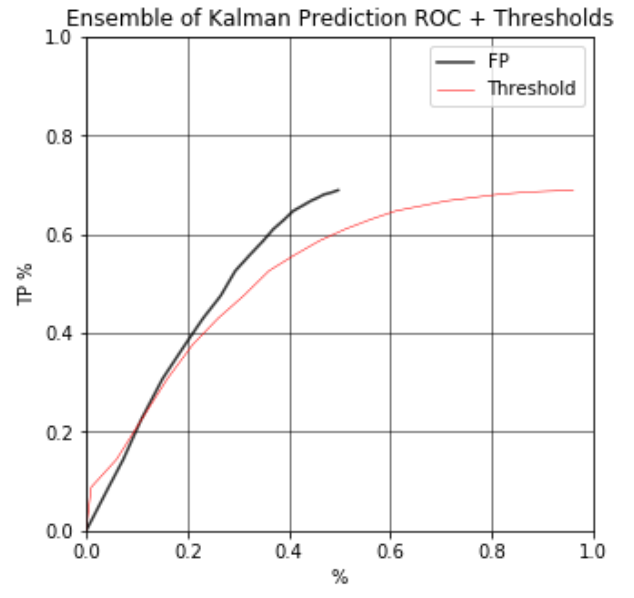
\includegraphics[width=6cm]{body/results/ensKF.png}
\caption{ROC generated based on an ensemble of random forests using kalman filter predictions on unscaled data.}
\label{fig:unKF}
\end{figure}

\begin{figure}[h]
\centering
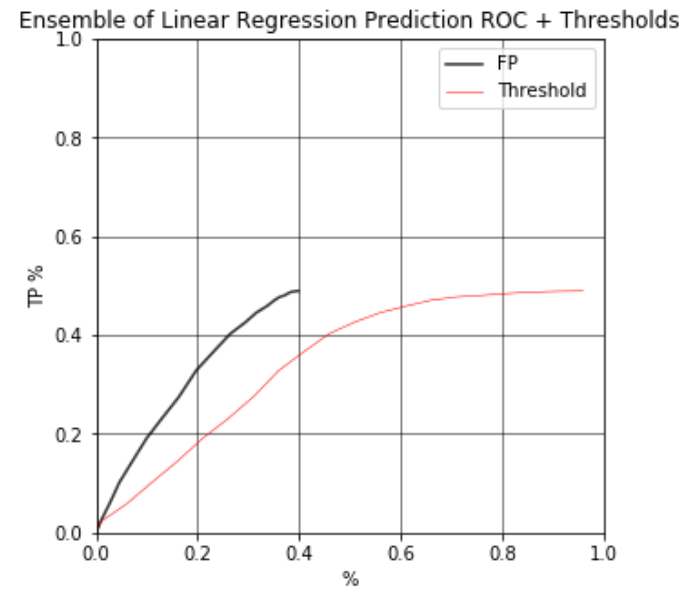
\includegraphics[width=6cm]{body/results/ensLR.png}
\caption{ROC generated based on an ensemble of random forests using least squares predictions on unscaled data.}
\label{fig:unLR}
\end{figure}
Figures \ref{fig:unKF} and \ref{fig:unLR} were generated based on the results of feeding the time series data into Kalman Filters (KF) and Least Squares Regressors (LR), respectively, with varying $Q$ and $\lambda$ parameters. Both the Kalman Filter and Linear Regression return $\alpha$ and $\beta$ parameters of the model $\alpha e^{\beta t}$. By plugging in the final time value for $t$, we computed the number of entries the contest is predicted to fill to. These predictions along with the $\alpha$ and $\beta$ parameters were used to train and test the Random Forest Classifier ensemble, represented by Figures \ref{fig:unKF} and \ref{fig:unLR}. Immediately, we can see that the ensemble of KF predictions appears to outperform the ensemble of LR predictions.
However, neither graphic seems to do too well, both falling short of even the basic baseline estimate from Figure \ref{fig:baseline}. 

Random Forests train by `binning' similar values and making predictions based on their collective success. We theorized that these classifiers might be more accurate if the values they were trained and tested on all shared the same range. As is, two contests with identical `shape' will result in different values of $\alpha$ and $\beta$ from the Kalman Filters and Linear Regressions. Additionally, the Predictions generated by the $\alpha$ and $\beta$ values will not be directly comparable. Take for example two contests of vastly different scales. Imagine contest 1 has a computed prediction of 1100 Entries and a goal of 1000, while contest 2 has a computed prediction of 110 Entries and a goal of 100 Entries. Even if the graphs for these two contests are  identical (except the axes of course), a random forest would be very unlikely to bin them together because the scale of their parameters would differ so widely. 

\begin{figure}[h]
\centering
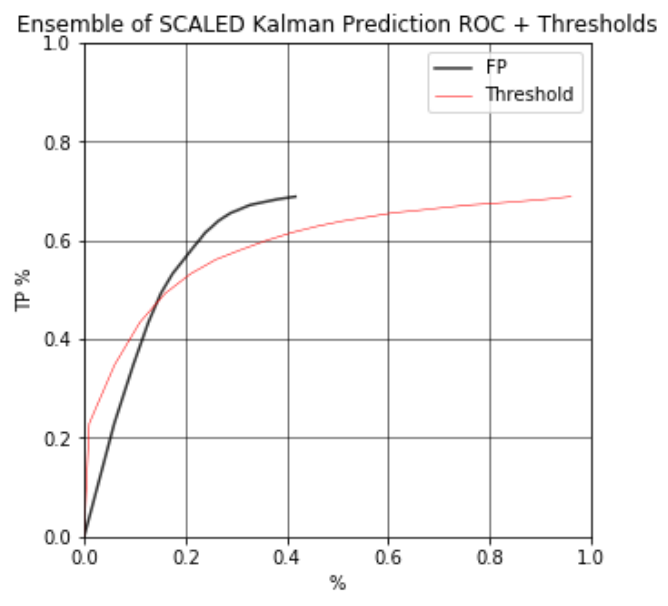
\includegraphics[width=6cm]{body/results/ensFKs.png}
\caption{ROC generated based on an ensemble of random forests using kalman filter predictions on scaled data.}
\label{fig:scaleKF}
\end{figure}

\begin{figure}[h]
\centering
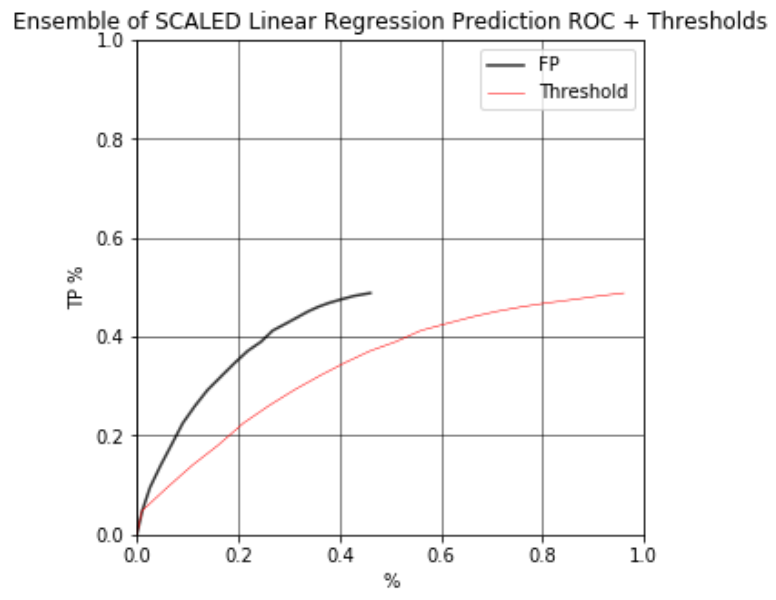
\includegraphics[width=6cm]{body/results/ensLRs.png}
\caption{ROC generated based on an ensemble of random forests using least squares predictions on scaled data.}
\label{fig:scaleLR}
\end{figure}

We hypothesized that scaling the time series data to a consistent domain in both time and total entries would enable a Random Forest Classifier to make more accurate predictions. Figures \ref{fig:scaleKF} and \ref{fig:scaleLR} show the resulting ROCs from performing KF and LR predictions on the data after scaling both axis to 100. In both cases, it seems scaling the data improves the overall predictive ability. Figure \ref{fig:allFits} shows a direct comparison of scaled outperforming unscaled predictions for both KF and LR ensembles.

\begin{figure}[h]
\centering
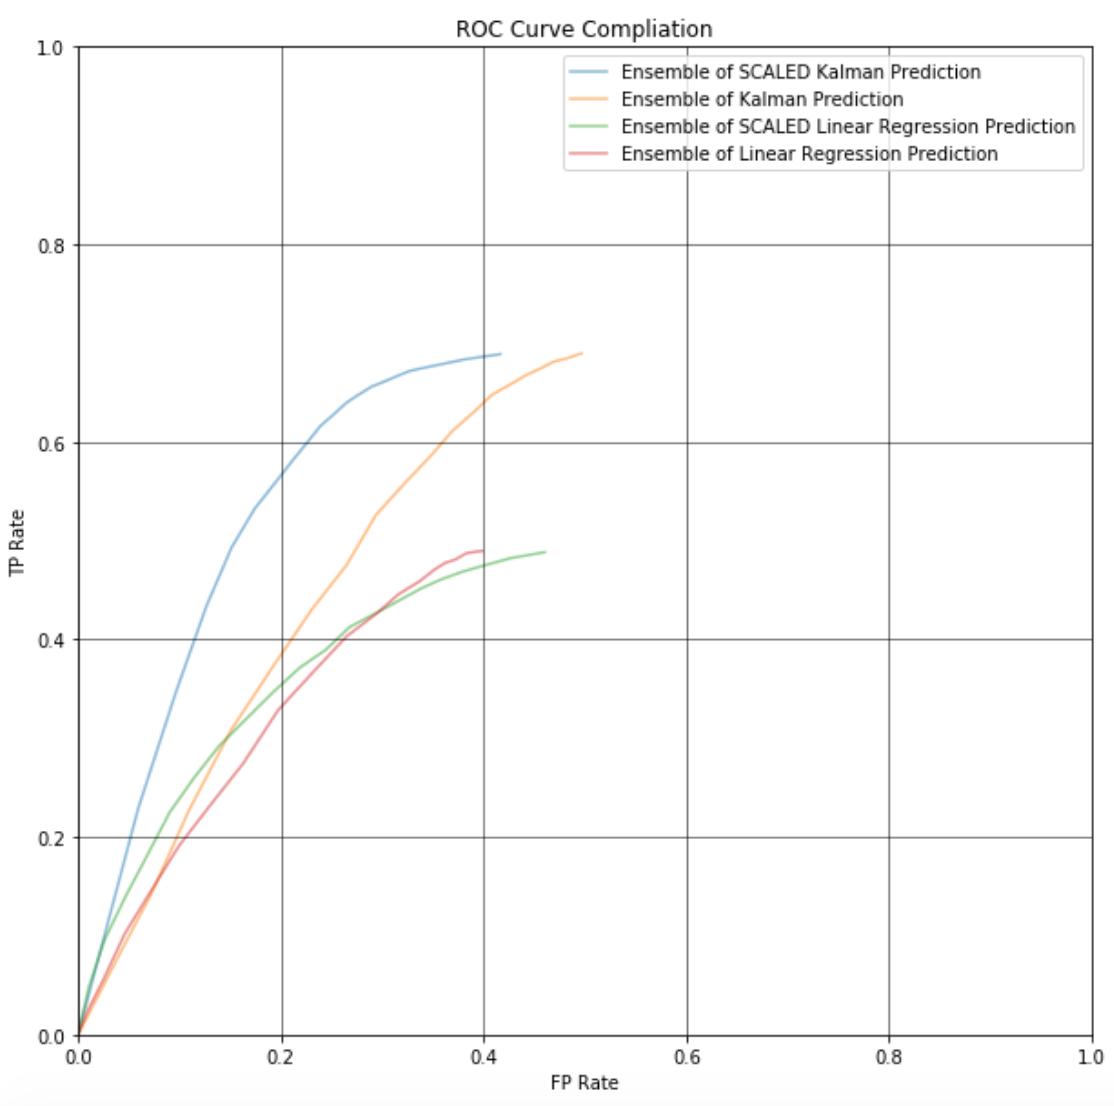
\includegraphics[width=6cm]{body/results/allEnsLines.png}
\caption{Comparison of predictive performances using our exponential model fitting methods on scaled and unscaled data in our ensemble.}
\label{fig:allFits}
\end{figure}

\begin{figure}[h]
\centering
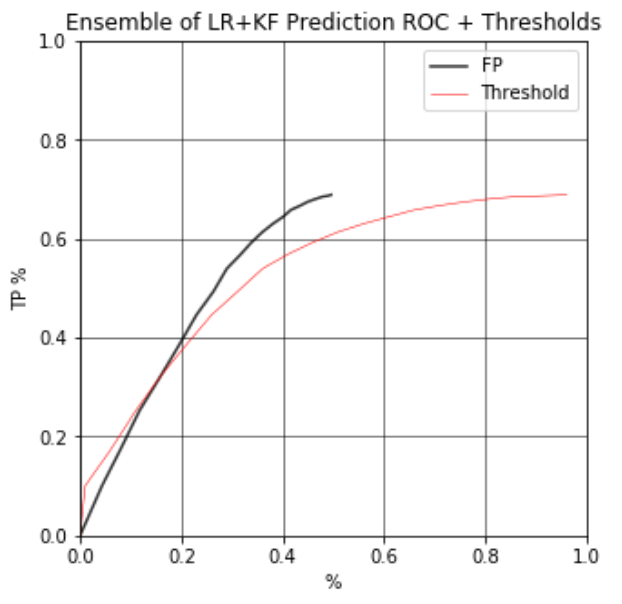
\includegraphics[width=6cm]{body/results/ensLR_KF.png}
\caption{ROC generated based on an ensemble of random forests using both kalman filter and least squares predictions on unscaled data.}
\label{fig:unBoth}
\end{figure}

\begin{figure}[h]
\centering
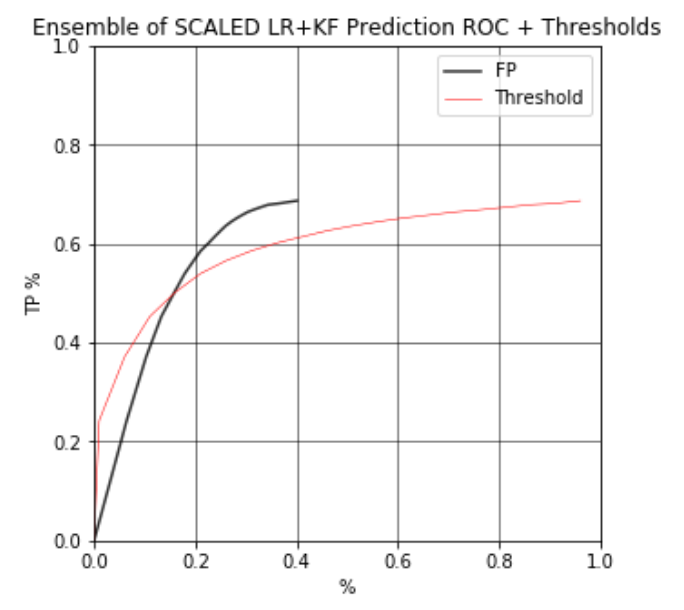
\includegraphics[width=6cm]{body/results/enLR_KFs.png}
\caption{ROC generated based on an ensemble of random forests using both kalman filter and least squares predictions on scaled data.}
\label{fig:scaleBoth}
\end{figure}

Both the Ensemble of Linear Regression and Kalman Filter results perform decently on their own, but our goal was to eventually make a single predictor (with a single ROC curve). By combining the results from Linear Regressions and Kalman Filter into a single RFC, we generated the ROC curves in Figures \ref{fig:unBoth} (using unscaled data) and \ref{fig:scaleBoth} (using scaled data). As would be expected given the last few results, the combined ensemble performed better when predicting on the scaled set of data. Again, a direct comparison of these two approaches can be seen in Figure \ref{fig:compCombo}.

\begin{figure}[h!]
\centering
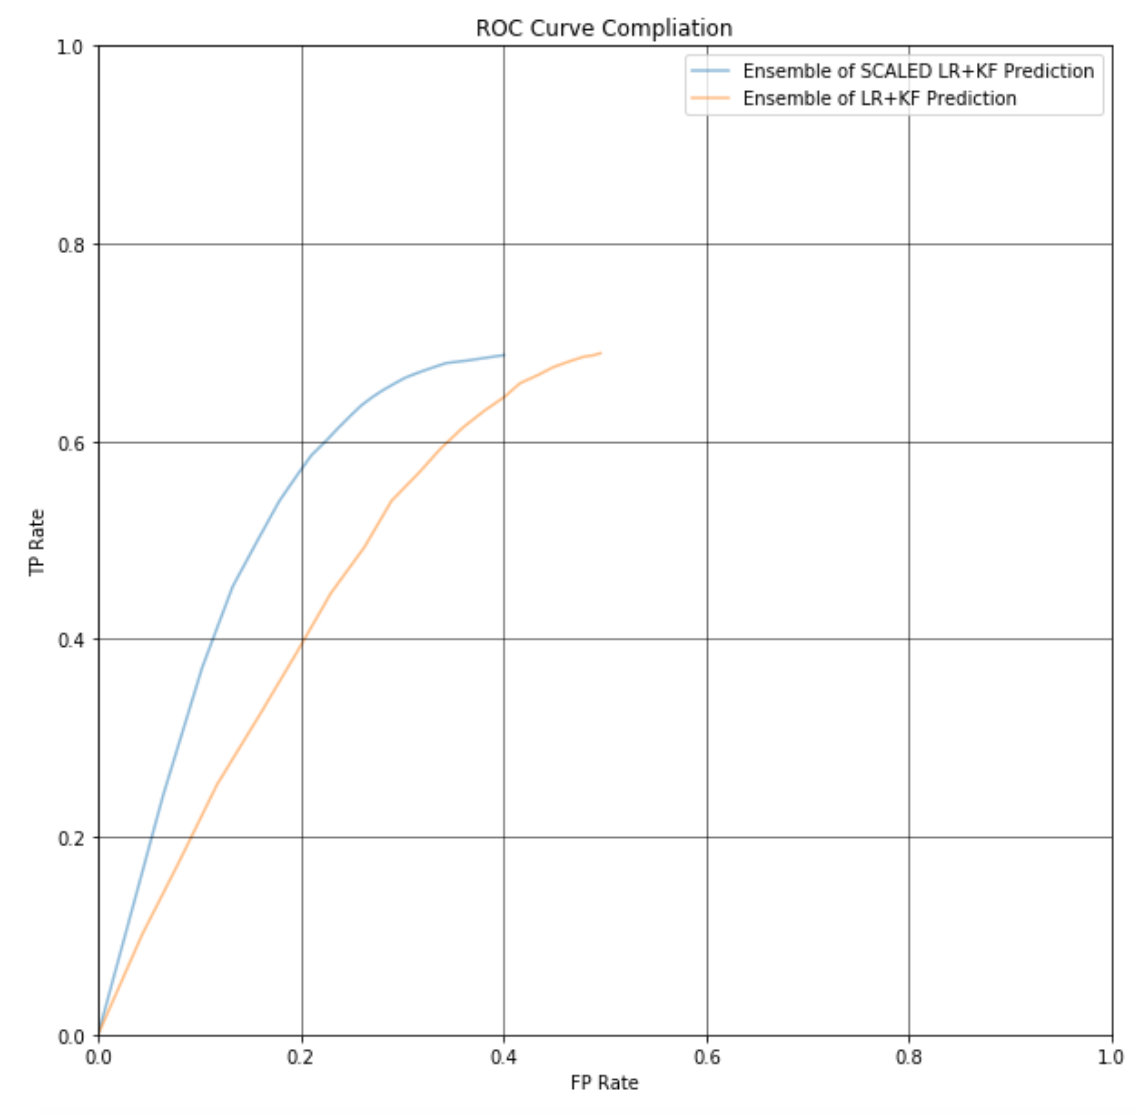
\includegraphics[width=6cm]{body/results/ensCombos.png}
\caption{Comparison of ROCs generated based on an ensemble of random forests using both kalman filter and least squares predictions on scaled and unscaled data.}
\label{fig:compCombo}
\end{figure}

 It's interesting here to note the similarities between the overall plots in Figures \ref{fig:scaleBoth} and \ref{fig:scaleKF}. Both seem to achieve a nearly 60\% true positive rate with only a 20\% false positive rate. On the whole, it seems using an ensemble of forests on both LR and KF on scaled data outperforms an ensemble of just KF on scaled data, but only minutely. This may indicate the KF is a superior predictor for this application over LR. Even still, at this point, this graphic only slightly outperforms the baseline metric from Figure \ref{fig:baseline}. However, now that we have a sufficiently strong ROC curve using only the Header Data and only the Time Series Data, it stands to reason that combining them should increase overall performance. 

\begin{figure}[h]
\centering
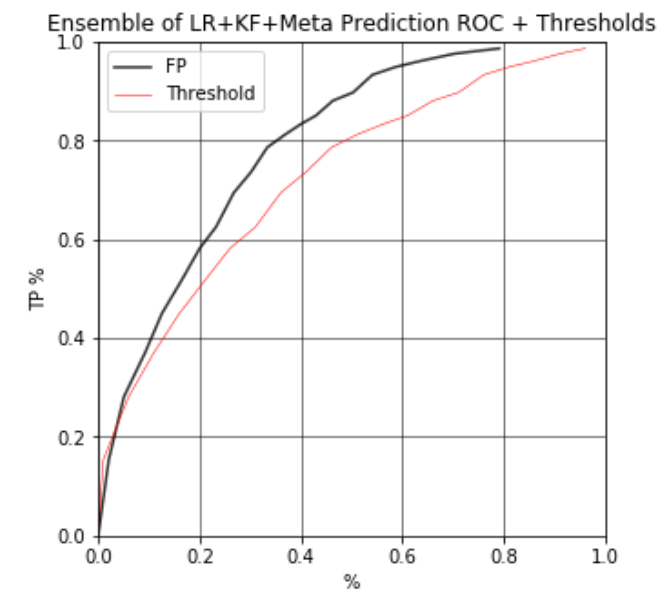
\includegraphics[width=6cm]{body/results/META_LR_KF.png}
\caption{ROC generated based on an ensemble of random forests using provided header data with both kalman filter and least squares predictions on unscaled data.}
\label{fig:MLRKF}
\end{figure}

\begin{figure}[h]
\centering
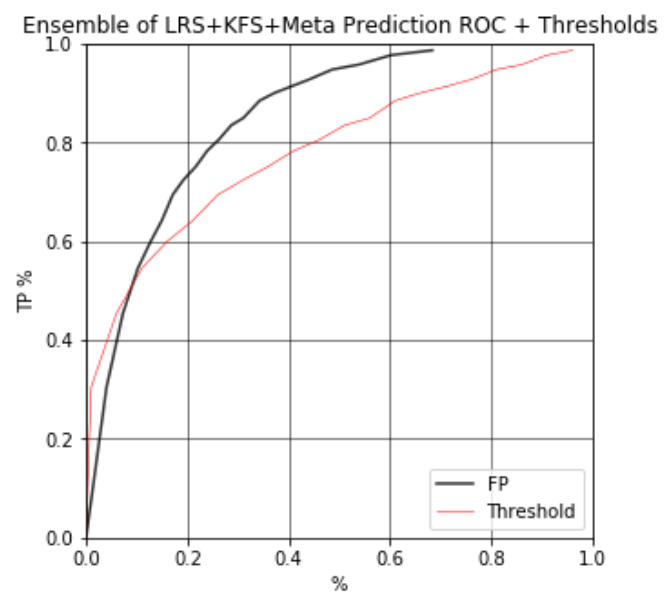
\includegraphics[width=6cm]{body/results/META_LR_KFs.png}
\caption{ROC generated based on an ensemble of random forests using provided header data with both kalman filter and least squares predictions on scaled data.}
\label{fig:MLRKFs}
\end{figure}

Figures \ref{fig:MLRKF} and \ref{fig:MLRKFs} are the the results of feeding the Linear Regression, Kalman Filter, and Header Data into a single ensemble with both scaled and unscaled data respectively. Once again, we can see scaling the data improves overall performance, particularly in the range from FP = 0.1 to 0.5. The direct comparison of the scaled and non-scaled versions is shown in Figure \ref{fig:MLRKFboth}. Comparing back to Figure \ref{fig:baseline} we can see that this approach seems to perform well, achieving an around 12\% better true positive rate over the baseline at the false positive point of 20\%. This is a significant improvement, however, comparing back to Figure \ref{fig:metaonly}, we can see that adding both KF and LR predictions to the ensemble only improves the same result by a few \% over the curve found using just the Header Data.

\begin{figure}[h]
\centering
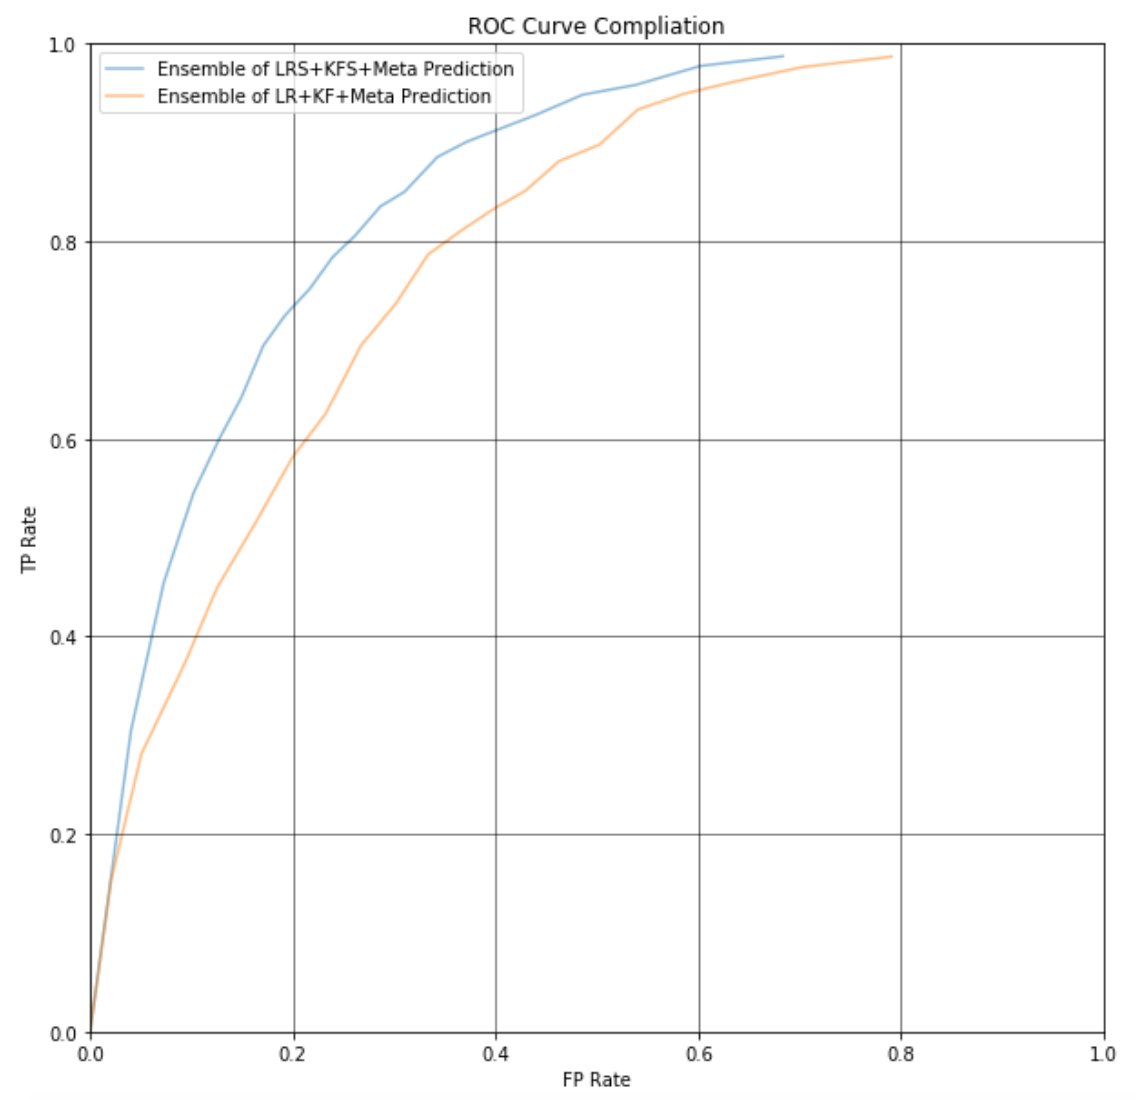
\includegraphics[width=6cm]{body/results/META_LR_KF_both.png}
\caption{Comparison of ROCs generated based on an ensemble of random forests using provided header data with both kalman filter and least squares predictions on scaled and unscaled data.}
\label{fig:MLRKFboth}
\end{figure}

\newpage
Up until now, the results would seem promising, however, the baseline comparison used so far is a rather low bar to strive for. Surely, if a classifier cannot outperform such a simple metric as ``Is the contest already full?'' then it is not worth the effort of designing. A better metric would be to see if the classifier can outperform the current predictive efforts being used by DraftKings themselves. Figure \ref{fig:pacer} shows the ROC created from the outputs of the currently implemented predictive algorithm at DraftKings, which we refer to as ``Pacer'' data. Comparing to Figure \ref{fig:MLRKFboth}, we can see the current Pacer estimates achieve around the same predictive performance as the ensemble of Header Data, Linear Regression, and Kalman Filter predictions on non-scaled data. However, we already know that scaling the data provides an even better result, so we can see this methodology even outperforms DraftKing's current Pacer estimates.

\begin{figure}[h]
\centering
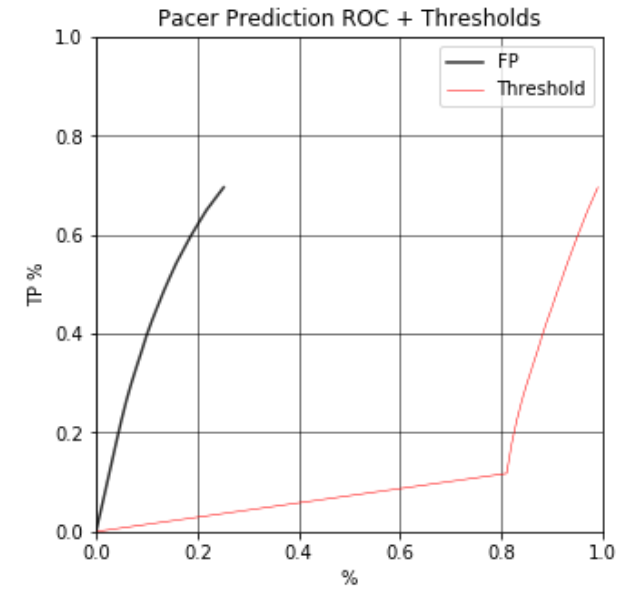
\includegraphics[width=6cm]{body/results/pacer.png}
\caption{ROC generated based on the predictive methods currently implemented at DraftKings.}
\label{fig:pacer}
\end{figure}

The observant reader may notice by now that adding more available data tends to improve the ensemble of Random Forests' predictions. Indeed, that is what we found tended to be the case. With that in mind, we would be remiss to not try adding in the current Pacer estimates into our ensemble with everything else to see what comes of it. As would be expected, this conglomerating seemed to outperform all other results discussed so far. Figure \ref{fig:everything} shows an overlay with many of the ``best so far'' results we've discussed to this point. For FP $\geq$ 0.15, the combined ensemble with Header, LR, KF, and Pacer data seems to achieve the highest TP rate. Interestingly though, for FP $\textless$ 0.15, it appears that an ensemble of just the Pacer and Header data does best.

\begin{figure}[h]
\centering
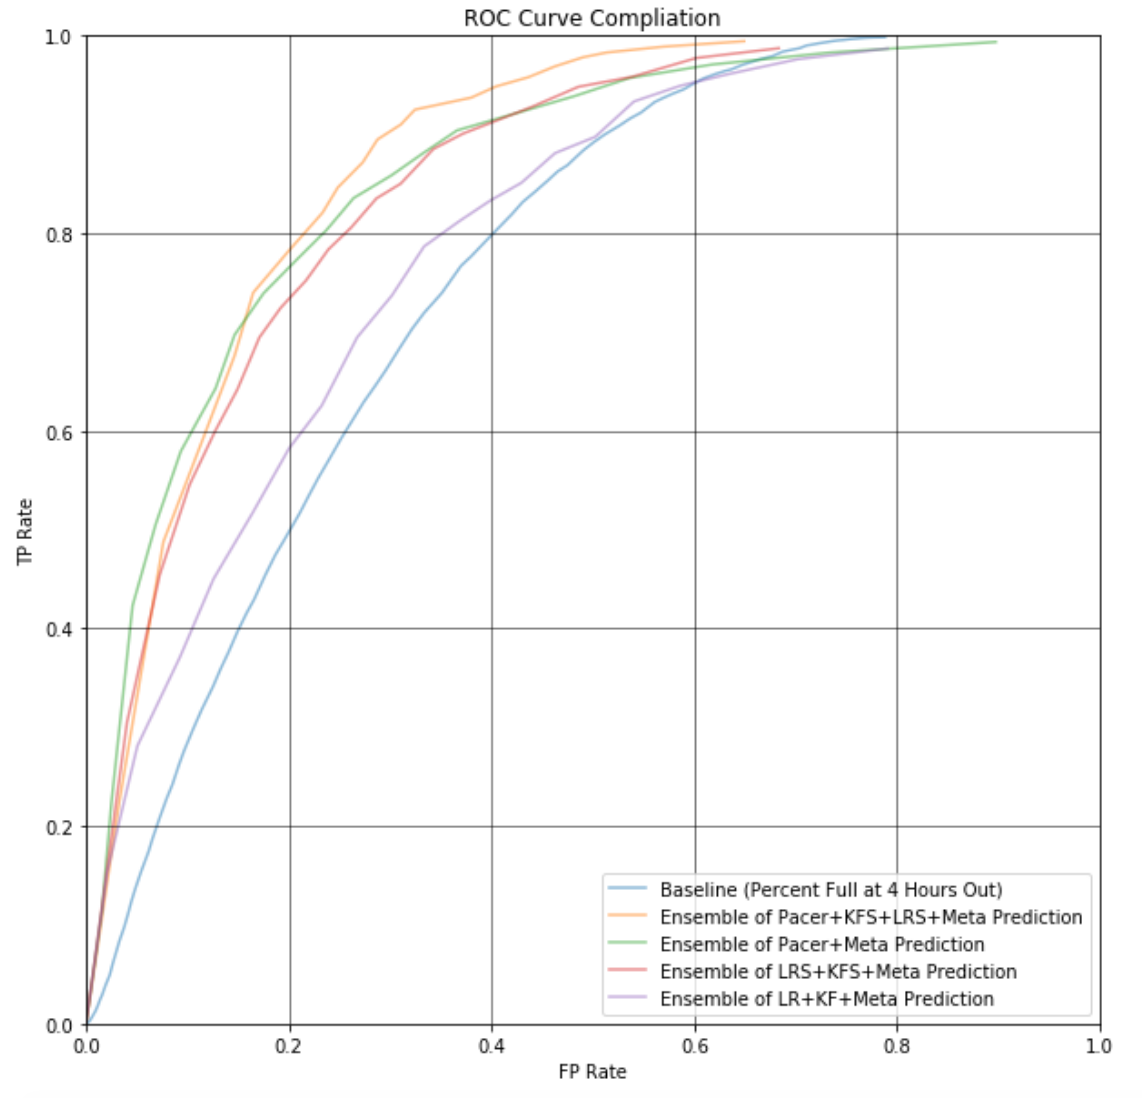
\includegraphics[width=6cm]{body/results/everything.png}
\caption{Comparison of ROCs generated using a variety of the methodologies outlined above.}
\label{fig:everything}
\end{figure}

\begin{figure}[h]
\centering
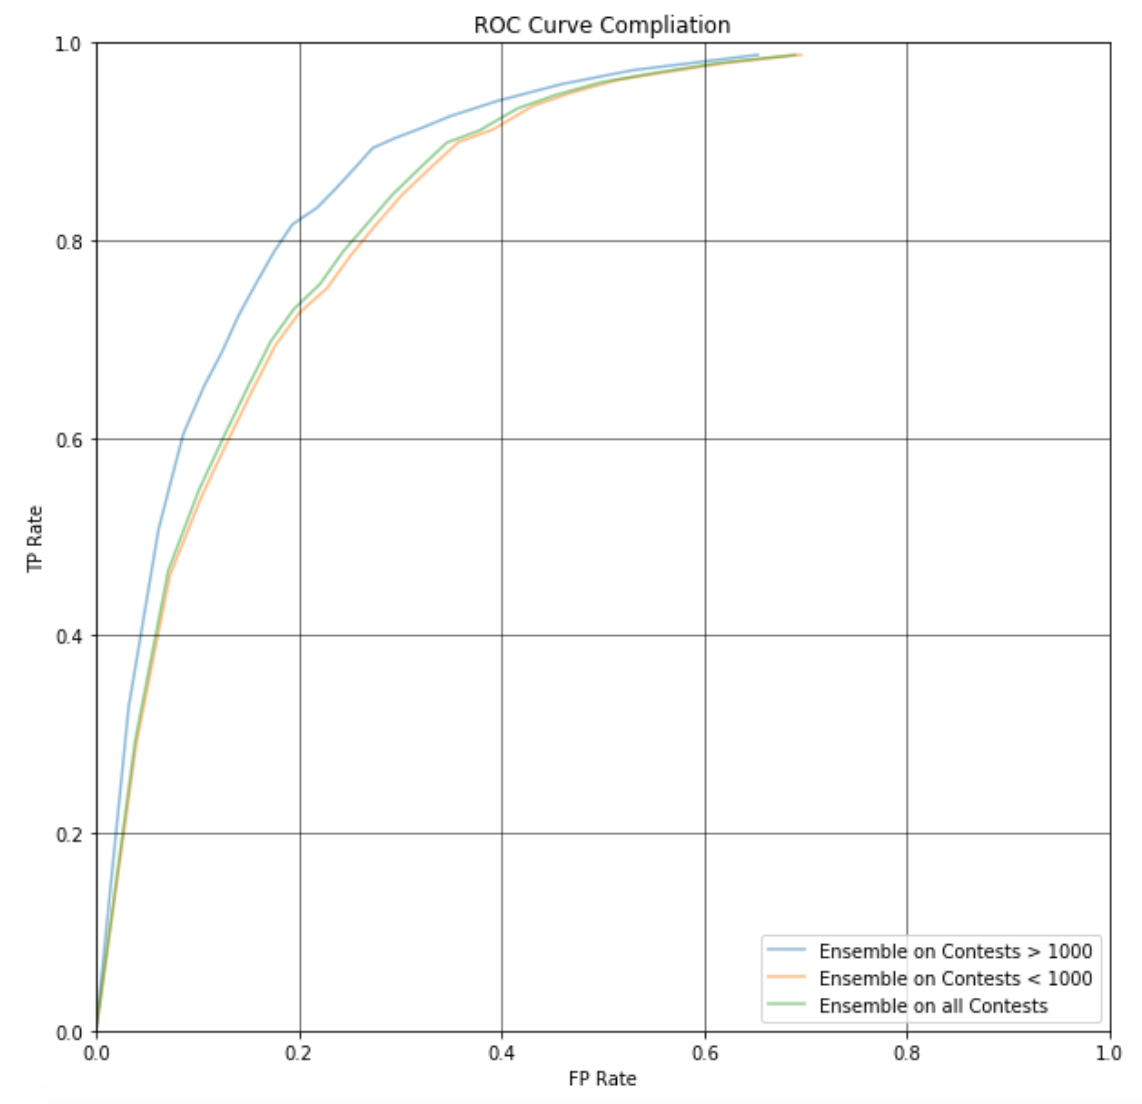
\includegraphics[width=6cm]{body/results/sizeSplit.png}
\caption{Comparison of ROCs generated based on an ensemble of random forests using Header, Pacer, kalman filter and least squares prediction data on just large (blue), just small (yellow) and all (green) contest respectively.}
\label{fig:sizeSplit}
\end{figure}

We found a large number of contests that were small tended to have little or no available time series data at the ``4 Hours Out'' mark which had negative effects on a lot of the KF and LR predictions. We decided to test if this had a significant affect on the overall curve. Figure \ref{fig:sizeSplit} shows the ROCs resulting from using the total conglomerated ensemble on just large (more than 1000 total  entries) and just small (less than 1000 total entries) contests. The ensemble seemed to perform better on larger contests, meaning the availability of more time series data may have a significant influence on our ability to predict. The prediction on small contests seemed to do only slightly worse than predicting on all contests. We believe this is because the majority of contests have little to no available time series data at ``4 Hours Out''. With this in mind, we opted to try a new approach.

Since the ROC in Figure \ref{fig:metaonly} was so successful without any Time Series data and the ROC for large contests only was even better, we wanted to try merging the two methods. To that end, we tried averaging the predictions of both ensemble methods. The resulting merged ROC can be found in Figure \ref{fig:averaged}. We can see that somehow, averaging the two methods achieves another significant improvement in the prediction. Comparing back to Figure \ref{fig:sizeSplit}, we see that the averaging method performs about equal to or better on all contest as the conglomerate method managed on just large contests. Relative to both previous success metrics from Figures \ref{fig:baseline} and \ref{fig:pacer}, the averaging methods appears to offer a drastically better prediction.

\begin{figure}[h]
\centering
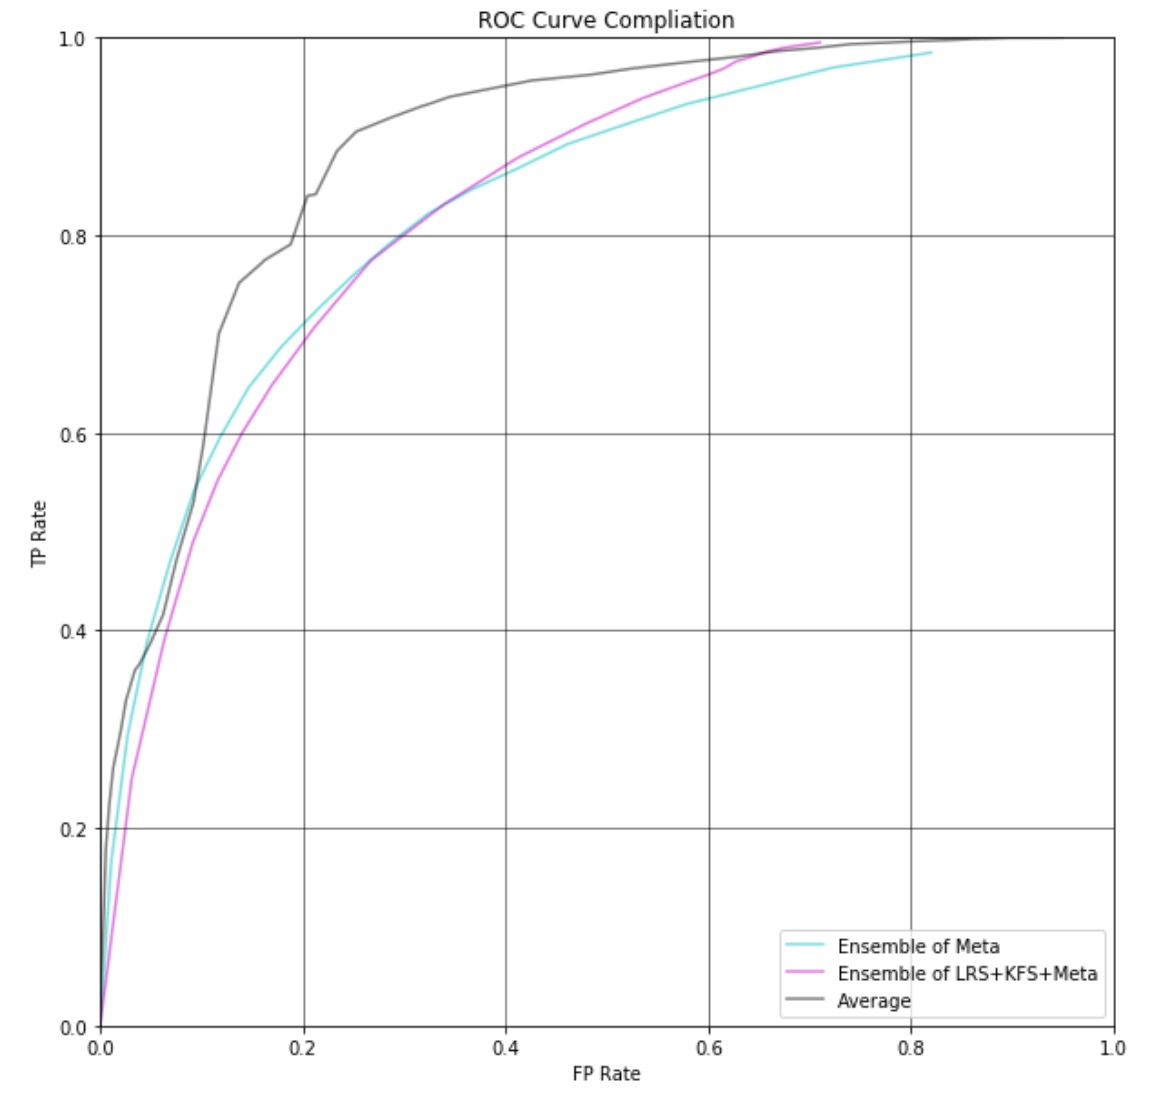
\includegraphics[width=6cm]{body/results/melded.jpeg}
\caption{Comparison of ROCs generated by an ensemble of random forests using Header, Pacer, kalman filter and least squares prediction data vs just using Header data vs an average of both.}
\label{fig:averaged}
\end{figure}

%one of the things Randy said about past drafts was that captions should be really detailed and even give some analysis, which I don't agree with, but the captions can be expanded. Also, I like the colorful graphs too, as I think it's easier to compare methods, so hopefully those are coming. Finally, I think the description of the results can be a little more example-based. Giving a point or two on the graph to describe can be really helpful for the reader to interpret the graphs better - JP